% !Mode:: "TeX:UTF-8"

\chapter{}
\textbf{
Decide whether you think the following statement is true or false. If it is true, give a short explanation. If it is false, give a counterexample.
}

\emph{Let G be an arbitrary flow network, with a source s, a sink t, and a positive integer capacity $c_e$ on every edge e; and let (A,B) be a minimum s-t cut with respect to these capacities $\{c_e:e\in E\}$. Now suppose we add 1 to every capacity; then (A,B) is still a minimum s-t cut with respect to these new capacities \{$1+c_e:e\in E$\}.}

\hspace*{\fill} \\
It is false. Let see the example in Fig~\ref{pic_5_1} and
Fig~\ref{pic_5_2}.
\begin{figure}[!htbp]
\centering
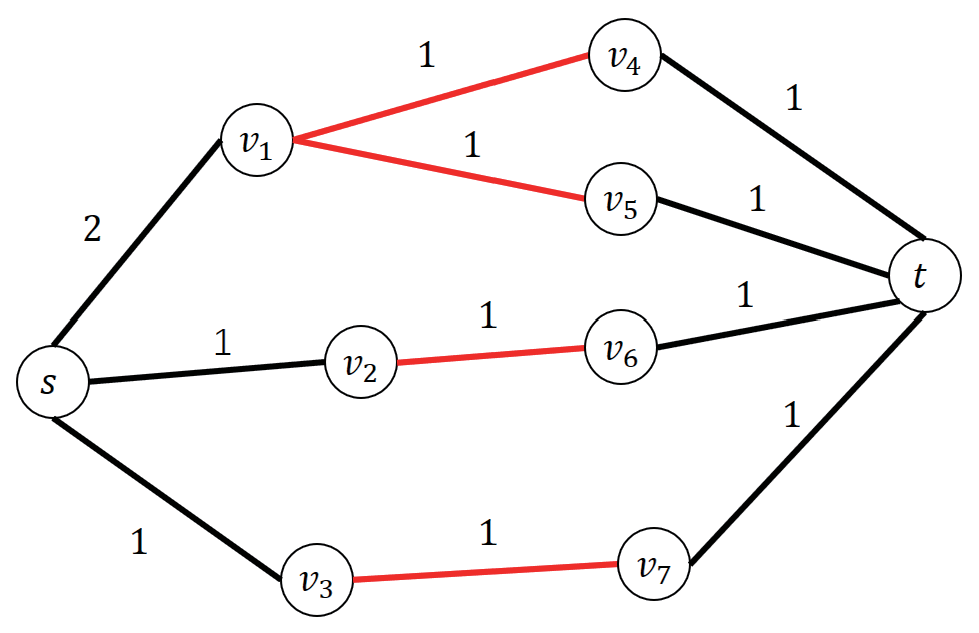
\includegraphics[width=0.5\textwidth]{figures/2.eps}
\caption{An example}\label{pic_5_1}
\end{figure}
We can see that in Fig~\ref{pic_5_1}, the red edges compose a cut. When we add 1 to each edge, it no more than a cut instead the cut is the composition of the red edges in Fig~\ref{pic_5_2}.
\begin{figure}[!htbp]
\centering
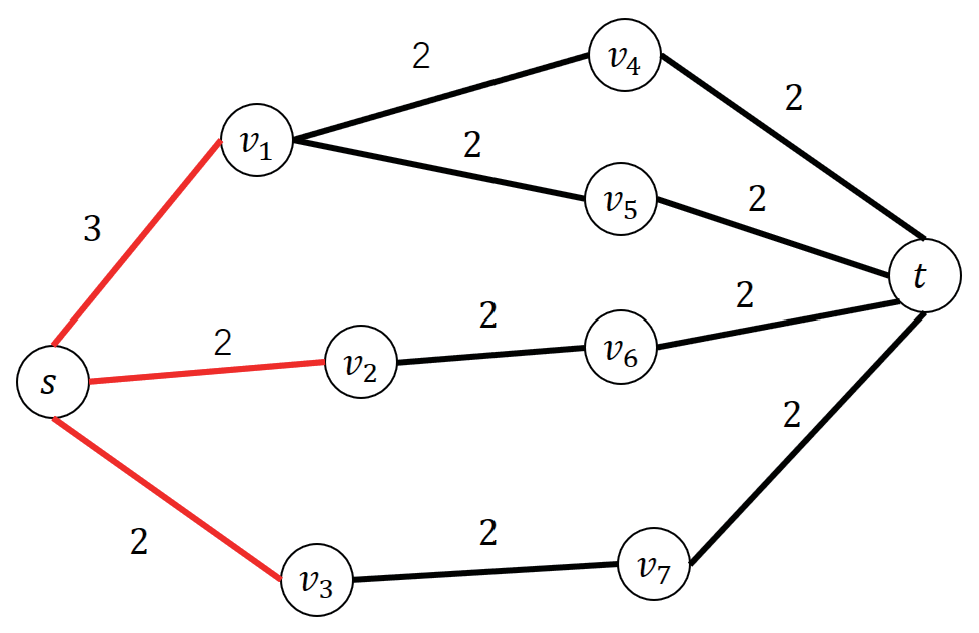
\includegraphics[width=0.5\textwidth]{figures/3.eps}
\caption{An example}\label{pic_5_2}
\end{figure}